%%%%%%%%%%%%%%%%%%%%
\chapter{Comparison and Results}
\label{cha:ComparisonAndResults}

This chapter presents the results that are achieved in the development of the FM Radio Receiver project, with the chosen different methods.
However, the main focus is to compare the results that are achieved with HLS and VHDL, since these are the major implementation variants of the project.

%%%%%%%%%%%%%%%%%%%%%%%%%%%%%%%%%%%%%%%%%%%%%%%%%%%%%%%%%%%%%%%%%%%%%%%%%%%%%%
\section{General}

A main objective of this thesis is to implement an FM radio receiver in multiple different methods.
This includes GNU Radio, Matlab, VHDL and HLS, which all have their advantages and disadvantages and surface different challenges to the developer.
The target functionality is to listen to the audio broadcast signal of an FM radio station.\\

All of the listed methods are implemented and the target functionality is achieved with all of them.
However, the level of detail that is required in the implementation, and the resulting effort and time it takes to implement the respective variant, differs by a large factor.
This is mainly due to the different levels of abstraction, so that the low-level algorithms do not need to be known.\\

In the following sections, especially the HLS and VHDL implementations are compared on the basis of metrics, but also based on the experience during development.


%%%%%%%%%%%%%%%%%%%%%%%%%%%%%%%%%%%%%%%%%%%%%%%%%%%%%%%%%%%%%%%%%%%%%%%%%%%%%%
\section{Functionality}

Generally, both tools -- HLS and VHDL -- provide the capabilities to implement any functionality in one or the other method.
However, the implementation is done in a different level.
VHDL uses an approach that is very close to the hardware, such as clock cycles and flipflops, while HLS describes the logic on an algorithmic level.\\

The implementation is split into two main parts, the communication interfaces and the DSP.
The results are presented in the following sections.

% Functionality same?
% DSP yes, AXI no (FSM of axi-stream)
% unit tests

%%%%%%%%%%%%%%%%%%%%
\subsection{Interfaces}

The AXI4-Lite memory-mapped bus is implemented to have an exactly equal behaviour in both variants.
There are read-only and read-writeable registers, which are all mapped onto a single base address.\\

The AXI stream interface however does not show the exact same behaviour.
Here, the HLS variant is using the AXI stream according to its protocol, while the VHDL variant is implemented differently.
It uses a simplified logic for the ready-flag, which reduces the effort in implementation.
However, from the perspective of the communicating blocks, the interface is usable like a regular AXI stream.
The implementation details are explained in Section \ref{sec:impl:vhdl:interfaces}.\\

In the final, integrated system on the SoC hardware, the CPU is able to communicate with both IPs via their interfaces successfully.
Status and configuration data can be read and written through the AXI4-Lite interface, and the streaming data for the DSP chain is successfully sent through the AXI streams as well.

%%%%%%%%%%%%%%%%%%%%
\subsection{Audio Output}

The audio output of the HLS and VHDL variants is compared with the Matlab model, which serves as the reference.
Additionally, the results of the testbench are compared with their respective result in the actual hardware.
In summary, it can be stated that the DSP chain produces a very similar audio output in all the compared data sets.
However, differences remain, which are presented in the following paragraphs and diagrams.

\includepicture [1.0] [0] {Comparison of the IP audio output signals, in simulation and hardware, against the Matlab model. The HLS variant matches the model, while the VHDL output diverts by a certain amount. Also, VHDL differs between simulation- and hardware results.} {audio_output_compare_tb_vs_hw} {img/matlab/audio_output_compare_tb_vs_hw}

%%%%%
\subsubsection{Comparing against the Matlab reference}

In the comparison against the Matlab model, the HLS variant achieves a very exact match of the output signal.
However, the VHDL implementation differs by a certain amount.
There seems to be an issue in the signal separation between the left and right audio channels.
This is visible in the analysis of the audio signal, as shown is Figure \ref{fig:audio_output_compare_tb_vs_hw}.
The signal strength of the left channel in the upper diagram is weaker than expected, while the right channel in the lower diagram is stronger.
This imbalance can also be observed by listening to the audio output via speakers.\\

The cause for this issue may be located in several components in the design.
This includes the FM demodulator, the carrier recovery, i.e. the 38~kHz carrier, as well as a sample timing shift in the final summation and substraction to recover the left and right channels.
The FIR filter has a successfully passing unit test and is thus assumed to be correct.
Also the fixed-point data type with its overflow- and rounding behaviour is suspected to be a potential issue.
Due to the time limitation in the elaboration of this thesis, this issue can not be traced down to the root cause and thus still persists in the current implementation.
However, from the system-level point of view of this thesis, the IP works and can be integrated into the final system.

%\includepicture [1.0] [0] {Comparison of the IP audio output signals against the Matlab model. The HLS variant matches the model, while the VHDL output diverts by a certain amount.} {audio_output_compare_ips_vs_matlab} {img/matlab/audio_output_compare_ips_vs_matlab}

%%%%%
\subsubsection{Comparing simulation- against hardware results}

Here, the results of the simulation testbenches are compared against the values that are read from the FPGA directly.
Ideally, the values should be exactly the same.
However, Figure \ref{fig:audio_output_compare_tb_vs_hw} shows that this is not always the case.
Again, the HLS implementation does have a matching result, whereas the VHDL variant has deviating values.
The explanation here may be linked with above suspicions, but may also be linked to the initial reset values that exist in the hardware.
In the HLS implementation, the reset logic of several registers is implemented automatically, whereas in VHDL these conditions need to be implemented manually.
Therefore, the IPs internal state, i.e. the register values, may be different at the beginning, which leads to an error propagation throughout the design.
The entire DSP chain is built like a pipeline and therefor it takes a number of samples to process, before the 'wrong' intermediate values are flushed out.
All that may be the cause for the deviating values in the VHDL design.\\

Again, the time limitation in the elaboration of this thesis does not allow a deeper analysis and investigation of this issue.
However, the end-to-end system design enables the developer to analyze an issue like this in a convenient way, in quick iterations.
Any adaptions in the VHDL design can be simulated and integrated into the FPGA with automated scripts.
Both results can then be analyzed and compared, which may lead to further adaptions.\\


%%%%%%%%%%%%%%%%%%%%%%%%%%%%%%%%%%%%%%%%%%%%%%%%%%%%%%%%%%%%%%%%%%%%%%%%%%%%%%
\section{Code Development}

In the development of a software project, the metric for the lines of code can be used to give an idea of the scale, or volume of the project.
The time it takes to implement a certain set of features can also give such an insight and a hint of the project's complexity.
It is a subjective metric though, since it is heavily influenced by the respective developer's experience in the specific application.
However, both metrics are applied to the FM Radio Receiver project.\\

At this point, it is important to note that the results that are presented in this section are very specific to the chosen architecture, testbench framework, and the implementation style generally.
Therefore, the numbers that are presented here may vary widely by modifying any of these factors, i.e. using a different testbench framework for VHDL.
Thus, a generalization in the art of \textit{HLS always requires less code than VHDL} can not be stated.
However, the results in this section can give an idea and overview of this topic and provide a detailed comparison for this specific project.

%%%%%%%%%%%%%%%%%%%%
\subsection{Lines of Code}

Several parts of the system design are taken into account to analyze the lines of code, to give an impression over the largest code parts in the project.
Figure \ref{fig:lines_of_code_pie_charts} shows multiple pie charts, which represent the proportions of the lines of code in the respective system design parts.
Table \ref{tab:lines_of_code} displays the actual numbers of code lines, to quantify the size of the respective parts.\\

Interesting details can be found by analyzing these charts.
The upper chart shows that the implementation of the hardware support, in the form of Vivado project scripts and the \cplusplus\ application software, takes a large part of the code with 27\%.
The remaining majority of the code belongs to the development of the IPs.
This includes the implementation of the Matlab model, the VHDL and HLS code, as well as the common testbench.
The chart also reveals that the VHDL implementation with its accompanying testbench requires more than twice the amount of code compared to the HLS version, i.e. 32\% versus 14\%.\\

The lower charts highlight several differences between HLS and VHDL.
Specifically, the code proportions between IP design and testbench are pointed out.
The charts show that HLS requires about the same amount of code for IP design and testbench.
VHDL requires the largest part of code in the IP design, while the testbench code amount is relatively small.
It is to be noted, that the common testbench consists of 4\%, which equals 630 lines of Python code.
Therefor, the testbench code of both IPs is relatively small, because the entire analysis part is shared.

\begin{figure}%
  \centering
  \subfloat[\centering Overview of the proportions between all the implemented code parts of the entire project.]{{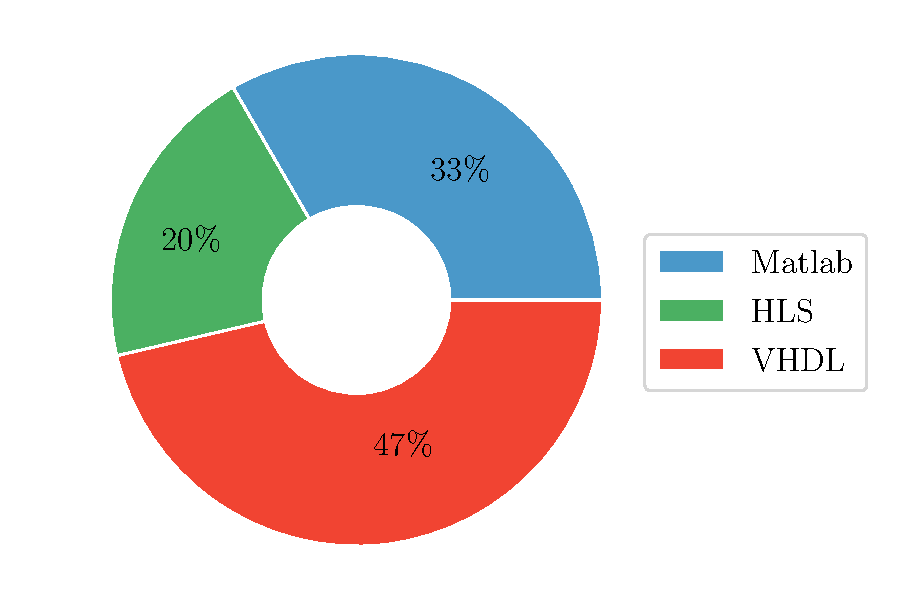
\includegraphics[trim=10 40 10 10,clip, width=0.65\textwidth]{img/matlab/lines_of_code_pie_chart_py_all} }}%
  \\
  %\hspace{\fill}
  \subfloat[\centering HLS in detail.]{{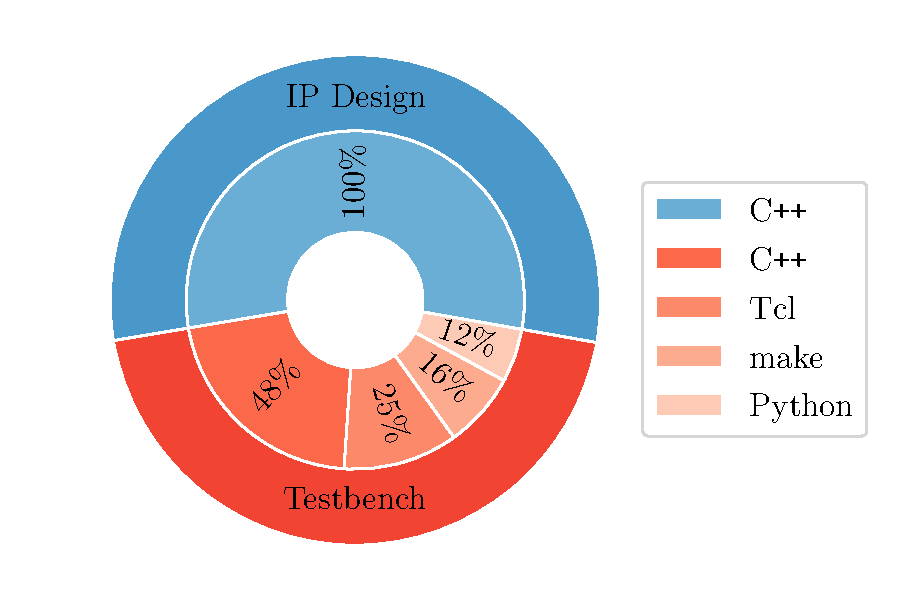
\includegraphics[trim=10 10 10 10,clip, width=0.49\textwidth]{img/matlab/lines_of_code_pie_chart_py_hls} }}%
  %\hspace{\fill}
  %\vspace{3cm}
  \subfloat[\centering VHDL in detail.]{{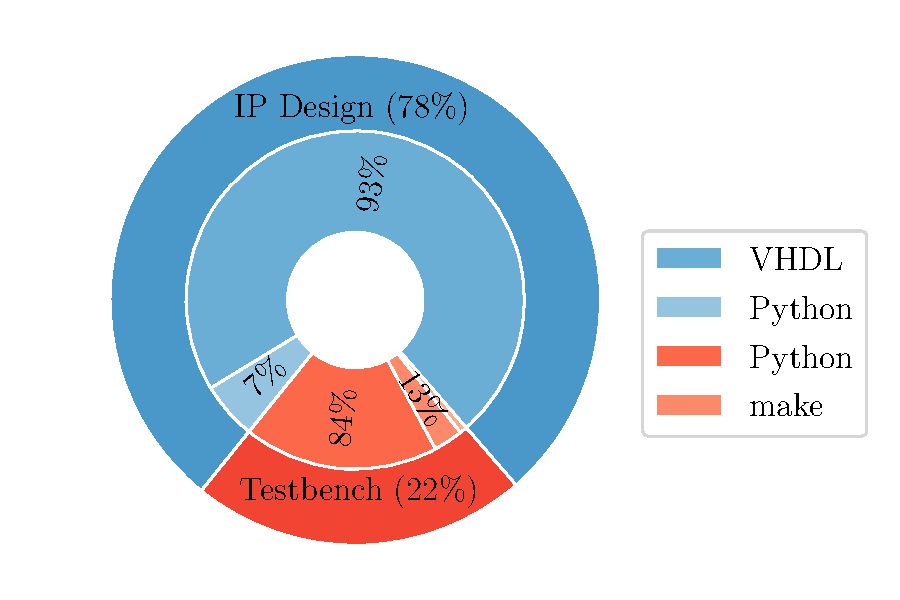
\includegraphics[trim=10 10 10 10,clip, width=0.49\textwidth]{img/matlab/lines_of_code_pie_chart_py_vhdl} }}%

  \caption{Lines of code of the respective code parts in the entire project, presented in multiple pie charts. The percentages of code in IP design and testbench for the HLS and VHDL implementations are shown in detail in the lower diagrams.}%
  \label{fig:lines_of_code_pie_charts}%
\end{figure}

\begin{table}[]
  \centering
  \begin{tabular}{l|c|c|}
  \cline{2-3}
  \textbf{}                                     & \multicolumn{1}{r|}{\textbf{IP Design}} & \multicolumn{1}{l|}{\textbf{Testbench}} \\ \hline
  \multicolumn{1}{|l|}{VHDL}                 & 3000                                    & 850                                     \\ \hline
  \multicolumn{1}{|l|}{HLS}                  & 920                                     & 740                                     \\ \hline
  \multicolumn{1}{|l|}{Common Testbench}        & \multicolumn{2}{c|}{630}                                                          \\ \hline
  \multicolumn{1}{|l|}{Matlab Model}            & \multicolumn{2}{c|}{2730}                                                         \\ \hline
  \multicolumn{1}{|l|}{Vivado Scripts}          & \multicolumn{2}{c|}{490}                                                          \\ \hline
  \multicolumn{1}{|l|}{\cplusplus\ Application} & \multicolumn{2}{c|}{2800}                                                         \\ \hline
  \end{tabular}
  \caption{The actual number of code lines, split in IP design and testbench, where applicable. All numbers are rounded up to tens.}
  \label{tab:lines_of_code}
\end{table}



%%%%%%%%%%%%%%%%%%%%
\subsection{Implementation Time}

% Implementation effort/time
%    -- see logged times; is subjective; had no previous knowledge
%    -- AXI interfaces --> huge effort in VHDL...
%        (mention Johannes Walter for generously providing/allowing the Register Engine script, adapted for this thesis)
%    -- drivers are auto-generated with HLS! huge time-saving..
%       (maybe show the code of AXI4-Lite interface and its generated driver
%        --> difference between R/W and RO!;
%        and show screenshots of the IP in the block design)

%%%%%%%%%%%%%%%%%%%%%%%%%%%%%%%%%%%%%%%%%%%%%%%%%%%%%%%%%%%%%%%%%%%%%%%%%%%%%%
\section{Simulation}
% Sim speed of x min of recorded FM signal
%
% VHDL:
%          time                samples
%   audio         sim        in      out
%  0.1000 s    73:44 min  (96000 -> 4000)
%  0.0100 s    09:37 min  ( 9600 ->  400)
%  0.0025 s    02:36 min  ( 2400 ->  100)
%
% HLS:



%%%%%%%%%%%%%%%%%%%%%%%%%%%%%%%%%%%%%%%%%%%%%%%%%%%%%%%%%%%%%%%%%%%%%%%%%%%%%%
\section{System Design}

The system design architecture that is chosen in this project covers several parts of the system.
This includes a reference model, the development of the IP itself, including the simulation testbench, as well as the final integration into the productive system.
Because of this structured approach, that is given by this system design, it can be applied to almost any DSP project.
The main processing IP can simply be replaced with another implementation, while the environment does not need to be modified.
The reason therefor is, that DSP projects almost always use streaming interfaces for their inputs and outputs.
Also a configuration interface is commonly used, to adapt certain parameters of the IP during runtime.


%%%%%%%%%%%%%%%%%%%%%%%%%%%%%%%%%%%%%%%%%%%%%%%%%%%%%%%%%%%%%%%%%%%%%%%%%%%%%%
\section{Deployment on Hardware}

%%%%%%%%%%%%%%%%%%%%
\subsection{Integration}
% IP generation and integration into Vivado

%%%%%%%%%%%%%%%%%%%%
\subsection{Hardware Utilization}
% --> utilization reports

%%%%%%%%%%%%%%%%%%%%
\subsection{Latency}
% --> utilization reports

%%%%%%%%%%%%%%%%%%%%%%%%%%%%%%%%%%%%%%%%%%%%%%%%%%%%%%%%%%%%%%%%%%%%%%%%%%%%%%
\section{Applicability}
% of all implementation variants
%   GNU Radio for fast prototyping,
%   Matlab for research
%   HLS/VHDL for deployment on HW, product development

